\subsubsection{Moving average filter}
Moving average filteret testes for at undersøge, hvorvidt de opstillede krav overholdes, samt undersøge om designet er korrekt implementeret. Måden, hvorpå dette testes er ved anvendelse af data fra pilotforsøget, da dette giver kontrolleret testforhold. 
En computer med MATLAB benyttes til at sende en givende måling til mikrokontrolleren, hvorpå det digitale filter er implementeret. Mikrokontrolleren returnerer løbende den filtrerede værdi, der visualiseres i MATLAB. Ud fra dette ses om filteteret virker hensigtsmæssigt. 
Resultatet af denne test fremgår af \autoref{fig:mavg_test}. 

\begin{figure}[H]
	\centering
	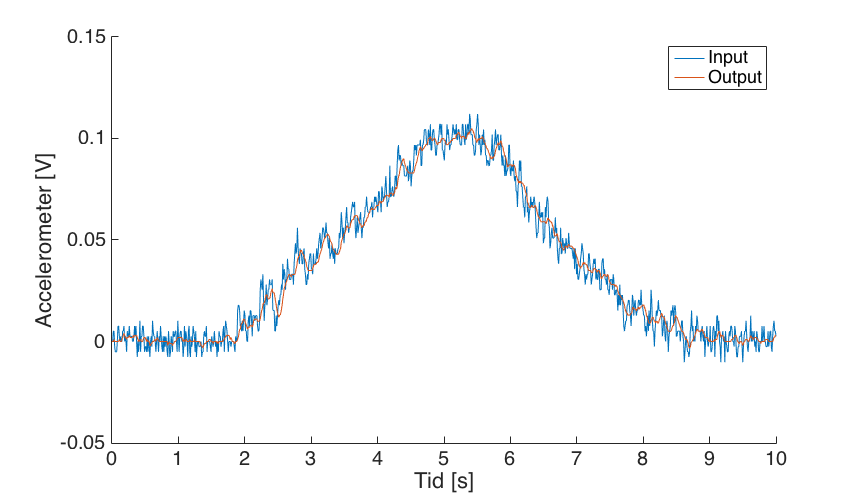
\includegraphics[width=1\textwidth]{figures/accelerometer_filter}
	\caption{Den blå graf illustrerer et ufiltreret signal fra accelerometer og den røde graf illustrerer et filtreret signal fra accelerometer, visualiseret i MATLAB}
	\label{fig:mavg_test}
\end{figure}

\noindent
Da filteret kræver 10 samples for at retunere den første værdi testes det, hvorvidt dette stemmer overens med det forventede forsinkelse på $100~ms$. Dertil er endnu en test foretaget, hvor et signal genereres i MATLAB. Dette signal sendes igen ind i mikrokontrolleren, hvortil et moving average filter pålægges. Herved er forsinkelsen beregnet. En visualisering af denne test ses af \autoref{fig:forsinkelse}

\begin{figure}[H]
	\centering
	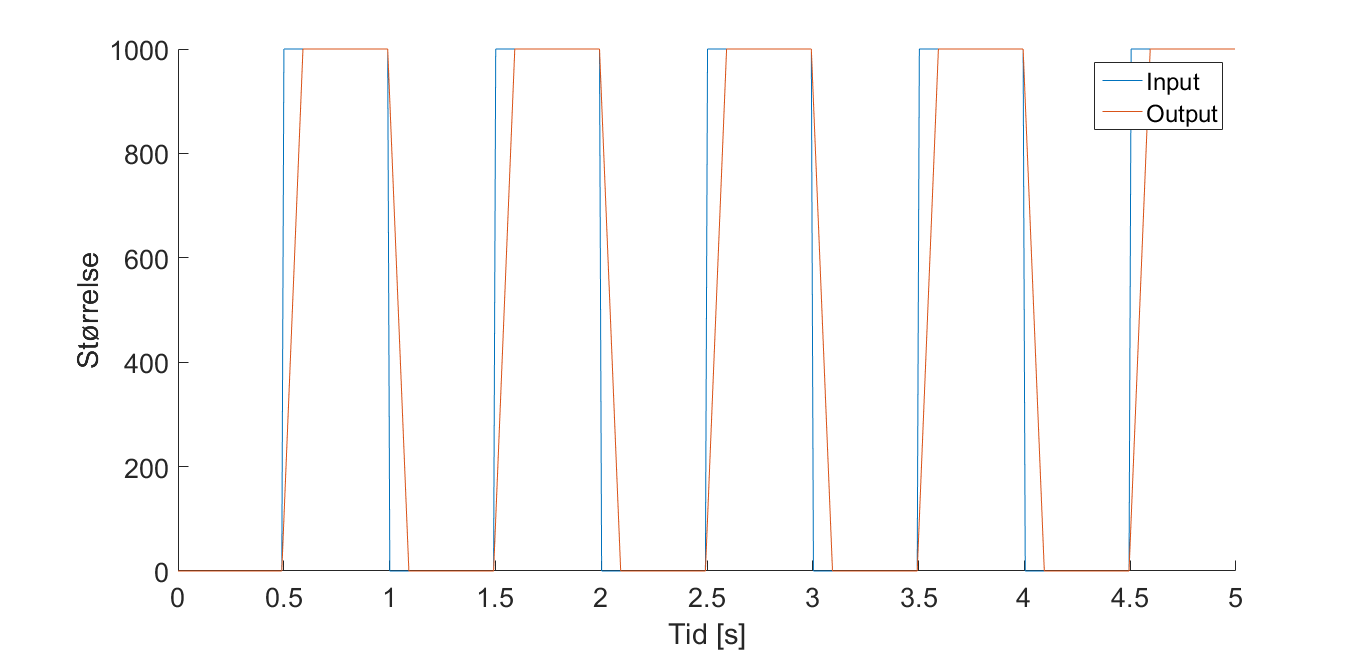
\includegraphics[width=1\textwidth]{figures/forsinkelse}
	\caption{Den blå graf illustrerer et ufiltreret signal, genereret i MATLAB og den røde graf illustrerer det filtreret signal, visualiseret i MATLAB}
	\label{fig:forsinkelse}
\end{figure}

\noindent
Resultatet fra denne test viser en forsinkelse af moving averge filteret på $0,09$ senkundt, hvilket er lavere end den forventede forsinkelse på $0,1$ sekundt og derfor accepteres. 

Yderligere foretages en test af forsinkelsen, der forekommer i det filteret eksekveres. Til denne test er en debug pin blevet defineret, hvor denne pin sættes som høj før funktionskaldet og lav efter funktionskaldet. Et oscilloscope tilsluttes debug pinen, således det kan måles, hvor længe debug pinen er høj. Resultatet fra testen er en forsinkelse på $320~\mu s$ for data at passere filteret. Dette betragtes som værende ikke af signifikant betydning.    
Ud fra ovenstående resultater vurderes det, at det filterede signal opfylder kravene for \autoref{sec:mavg_krav}. 


\vspace{3mm}
\textbf{Opsummering af krav:}
\begin{itemize}
\item[\text{\sffamily \checkmark}] Skal muliggøre en repræsentation af spændinger 
\item[\text{\sffamily \checkmark}] Skal have en filterlængde på $10$ samples
\item[\text{\sffamily \checkmark}] Skal have en maksimal forsinkelse på $100~ms$
\end{itemize}